\documentclass[dvipdfmx,tikz]{standalone}
\usepackage{tikz}
\usetikzlibrary{intersections}
\begin{document}
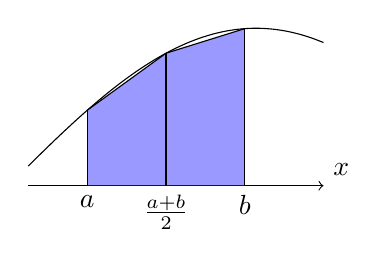
\begin{tikzpicture}[domain=0.25:4]
%\draw[help lines] (0,0) grid (8,-12);
\path[draw,->,thin] (0.25, 0) -- (4,0) node[above right] {$x$};
%\path[draw,->] (0, -1) -- (0,2) node[right=2mm] {\large $y$};

\coordinate (a) at (1,0);
\coordinate (up_a) at (1,{2*sin(0.5 r)});
\coordinate (b) at (3,0);
\coordinate (up_b) at (3,{2*sin(1.5 r)});
\coordinate (middle) at (2,0);
\coordinate (up_middle) at (2,{2*sin(1 r)});

\fill[blue!80!white,opacity=.5] (a) -- (up_a) -- (up_middle) -- (up_b) -- (b) -- (a);

\node[below] at (a) {$a$};
\draw[thin] (a) -- (up_a);
\node[below] at (b) {$b$};
\draw[thin] (b) -- (up_b);

\node[below] at (middle) {$\frac{a+b}{2}$};
\draw[thin] (middle) -- (up_middle);

\draw[thin] (up_a) -- (up_middle);
\draw[thin] (up_b) -- (up_middle);

\draw[color=black,smooth,thin] plot(\x,{2*sin(\x/2 r)})node[right] {};
\end{tikzpicture}
\end{document}